\documentclass[oneside, 11pt, notitlepage, a4paper, numbers=noenddot]{scrartcl}

\usepackage{thisemi}
\usepackage[pdftex]{graphicx}

\title {Analyse von PST-Dateien}
\author{Alexander Pilz}
\date  {Sommersemester 2022}

\begin{document}

\maketitle

\section{Einleitung}
E-Mails sind im privaten wie auch im geschäftlichen Umfeld nicht mehr als Kommunikationsmedium wegzudenken. Dies ist klar erkennbar an den versandten und empfangenen E-Mails weltweit. So lag diese Zahl im Jahr 2021 bei 319,6 Milliarden E-Mails und steigt laut einer Prognose bis ins Jahr 2025 auf 376,4 Milliarden E-Mails \cite{Statista.26.06.2022}. 

E-Mails werden heutzutage aber nicht nur für die Kommunikation verwendet, sondern auch zum Versenden von Spamnachrichten. So beläuft sich der Anteil an Spam-Mails am weltweiten Anteil der versandten E-Mails auf 46 Prozent \cite{ASITZentrumfursichereInformationstechnologieAustria.26.06.2022}. Unter Spam versteht man Nachrichten, die ohne Aufforderung und unterwünscht zugestellt werden. Meist haben diese Nachrichten den Zweck Werbung zu verbreiten. Jedoch gibt es auch weitaus bedenklichere Nachrichten. So wird mithilfe von Spam-Mails versucht, unvorsichtige Nutzer dazu zu bringen, persönliche Daten preiszugeben oder finanzielle Gewinne zu erzielen. 

Im geschäftlichen Umfeld wird hier dem Nutzer meist die Arbeit abgenommen, weil professionelle Spam-Filter eingerichtet sind und so fast keine unerwünschten Nachrichten mehr ankommen. Im privaten Umfeld werden solche Spamfilter oft nicht bzw. nicht richtig angewandt. Hinzu kommt, dass sich viele Nutzer mit dieser Thematik gar nicht auseinandersetzen. Dies führt häufig dazu, dass die Postfächer der Nutzer hier regelrecht durch Spam-Mails überladen werden. 

Im Rahmen dieser Seminararbeit sollen diese unerwünschten E-Mails mithilfe des .PST-Dateiformats analysiert und die Ergebnisse dokumentiert werden.
\newpage
\label{Einleitung}

\section{Allgemeines}


\label{Allgemeines}

\section{PST-Datei}
\noindent Das .pst-Dateiformat ist ein proprietäres Dateiformat, welches von Microsoft im Mailprogramm \glqq{}Outlook\grqq{} verwendet wird. PST steht dabei für Personal Storage Table. Microsoft nutzt das Dateiformat zum Speichern von Nachrichtenkopien, Kalendereinträgen und Kontakten. Nutzt man den Microsoft Exchange Server werden die Daten an den Server übermittelt und dort gespeichert. Im Gegensatz dazu speichert Microsoft Outlook ohne Exchange Server diese Elemente auf dem lokalen Computer. Dabei werden .pst-Dateien meist zum Speichern archivierter Elemente verwendet. \smallskip

\noindent Zum besseren Verständnis kann eine .pst-Datei auch als ein \glqq{}Aktenschrank\grqq{} bzw. eine \glqq{}Büroablage\grqq{} bezeichnet werden. Diese besitzt beschriftete Schubladen, in denen die verschiedenen Daten kategorisch sortiert abgelegt werden. Hängen diese übergreifend miteinander zusammen, besteht die Möglichkeit Querverweise zwischen den einzelnen Schubladen herzustellen. Der genaue Aufbau dieser Architektur wird im nächsten Abschnitt dieser Arbeit näher erläutert. Die PST-Dateien sind gewöhnlich nur mit Outlook zu öffnen, jedoch gibt es mittlerweile auch andere Tools um diese zu öffnen, bzw. zu analysieren. Auf diese Tools wird an dieser Stelle nicht weiter eingegangen, da ich diese nicht verwendet habe.
\label{PST-Datei}

\subsection{Aufbau einer PST-Datei}
Der Aufbau einer PST-Datei ist in Abbildung \ref{fig:pstarchitecture} abgebildet. Er besteht aus drei Schichten:

\begin{itemize}
    \item Messaging Layer
    \item LTP Layer (Lists, Tables, and Properties)
    \item NDB Layer (Node Database)

\end{itemize}

Aus der Dokumentation des .pst-Dateiformats kann folgendes entnommen werden: \newline
Die Messaging Layer besteht aus den übergeordneten Regeln und der Geschäftslogik, die es ermöglichen, die Strukturen der LTP- und NDB-Schichten zu kombinieren und als Ordnerobjekte, Nachrichtenobjekte, Attachment-Objekte und Eigenschaften zu interpretieren. Die Messaging-Schicht definiert auch die Regeln und Anforderungen die beim Ändern des Inhalts einer PST-Datei befolgt werden müssen, damit die geänderte PST-Datei weiterhin erfolgreich von Implementierungen dieses Dateiformats gelesen werden kann. \newline
Die LTP-Schicht implementiert übergeordnete Konzepte auf dem NDB-Konstrukt. Die Kernelemente der LTP-Schicht sind der Property Context (PC) und der Table Context (TC). Ein PC repräsentiert eine Sammlung von Eigenschaften. Ein TC stellt eine zweidimensionale Tabelle dar. Die Zeilen stellen eine Sammlung von Eigenschaften dar. Die Spalten geben an, welche Eigenschaften in den Zeilen enthalten sind.
Vom Standpunkt einer High-Level-Implementierung aus gesehen, wird jeder PC oder TC als Daten in einem einzelnen Knoten gespeichert. Die LTP-Schicht verwendet NIDs, um PCs und TCs zu identifizieren.\newline
Um PCs und TCs effizient zu implementieren, verwendet die LTP-Schicht die folgenden zwei Arten von Datenstrukturen über jedem NDB-Knoten.
Die NDB-Schicht besteht aus einer Datenbank von Knoten, die die untergeordneten Speichermöglichkeiten des PST-Dateiformats darstellt. Aus der Sicht der Implementierung besteht die NDB-Schicht aus dem Header, den Dateizuordnungsinformationen, Blöcken, Knoten und zwei BTrees: dem Node BTree (NBT) und dem Block BTree (BBT). Der NBT enthält Verweise auf alle zugänglichen Knoten in der PST-Datei. Seine BTree-Implementierung ermöglicht eine effiziente Suche nach einem bestimmten Knoten. Jeder Knotenverweis wird durch einen Satz von vier Eigenschaften dargestellt, die seine NID, übergeordnete NID, Daten-BID und Unterknoten-BID umfassen. Die Daten-BID verweist auf den Block, der die mit dem Knoten verbundenen Daten enthält, und die Unterknoten-BID verweist auf den Block, der Verweise auf Unterknoten dieses Knotens enthält. Die NIDs der obersten Ebene sind im gesamten PST eindeutig und können von der NBT aus durchsucht werden. Unterknoten-NIDs sind nur innerhalb eines Knotens eindeutig und können nicht über die NBT gesucht (oder gefunden) werden. Die übergeordnete NID ist eine Optimierung für die höheren Schichten und hat keine Bedeutung für die NDB-Schicht. Der BBT enthält Verweise auf alle Datenblöcke der PST-Datei. Seine BTree-Implementierung ermöglicht eine effiziente Suche nach einem bestimmten Block. Ein Blockverweis wird durch einen Satz von vier Eigenschaften dargestellt, zu denen seine BID, IB, CB und CREF gehören. IB ist der Offset innerhalb der Datei, an dem sich der Block befindet. CB ist die Anzahl der im Block gespeicherten Bytes. CREF ist die Anzahl der Verweise auf die im Block gespeicherten Daten. Auf die Wurzeln der NBT und BBT kann über den Header der PST-Datei zugegriffen werden.
Das folgende Diagramm \ref{fig:nodesblockspst} veranschaulicht die Beziehung zwischen Knoten und Blöcken auf hoher Ebene \cite{.c}.

\begin{figure}
    \centering
    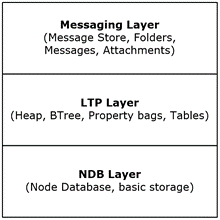
\includegraphics[width=0.50\textwidth]{images/PST_File.png}
    \caption{Logische Architektur einer PST-Datei \cite{.c}} 
    \label{fig:pstarchitecture}
\end{figure}

\begin{figure}
    \centering
    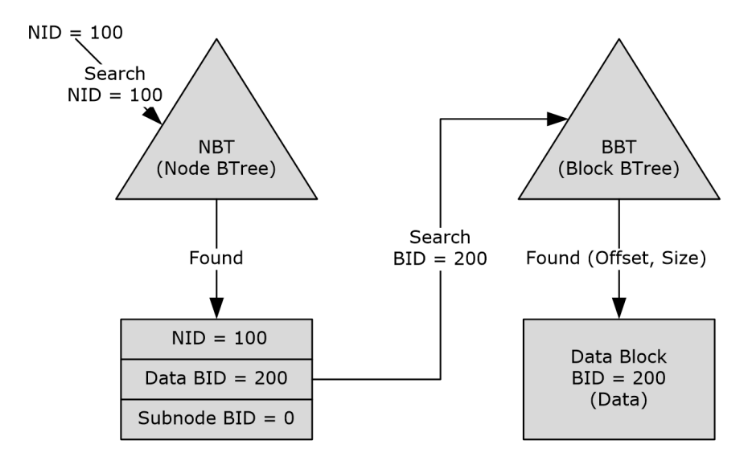
\includegraphics[width=0.75\textwidth]{images/nodes_blocks_pst.PNG}
    \caption{Beziehung zwischen Knoten und Blöcken \cite{.c}} 
    \label{fig:nodesblockspst}
\end{figure}
\label{Aufbau einer PST-Datei}

\subsection{Sicherheitsprobleme mit PST-Dateien}
PST-Dateien bieten den Vorteil, dass sie leicht übertragbar sind. Auch ohne fundierte IT-Kenntnisse können sie zwischen verschiedenen Outlook-Clients übertragen werden. Abgesehen von diesem Mobilitätsvorteil bringen sie jedoch auch Sicherheitsprobleme mit sich \cite{.26.06.2022}:

\begin{itemize}
    \item Beschädigungs- bzw. fehleranfällig, was zu Datenverlusten führen kann
    \item Stromausfälle, PC-Abstürze oder versehentliches Schließen trennen eine PST-Datei vom Outlook-
    Profil (abgekoppelte oder verwaiste PSTs entstehen, die für die IT-Abteilung nicht sichtbar sind,
    auch wenn sie wertvolle Informationen enthalten, die benötigt werden)
    \item Inhalte von PST-Dateien sind nur an der Quelle verfügbar und somit bei Analysen von zentralen Punkten aus eventuell nicht verfügbar
    \item Zugangsbeschränkungen oder eine falsche Klassifizierung können dazu führen, dass PST-Objekte
    falsch kategorisiert werden
    \item Passwortschutz vorhanden, kann aber sehr leicht entschlüsselt werden
    \item Native PST-Verschlüsselung bietet keinen ausreichenden Schutz
\end{itemize}
\label{Sicherheitsprobleme mit PST-Dateien}

\section{Schritte bei der Analyse der PST-Datei}
In diesem Kapitel werden die durchgeführten Analyseschritte näher erläutert. Dabei wird auf eine Senderanalyse, eine zeitliche Analyse sowie eine Analyse bestimmter Schlagwörter eingegangen.
\label{Schritte bei der Analyse der PST-Datei}

\subsection{Datensatz}
Zuerst wird näher auf den verwendeten Datensatz für die Analyse eingegangen. Dabei war die Auswahl eines geeigneten Datensatzes schwieriger als anfangs erwartet, da der Datensatz auch bestimmte Kriterien für die Analyse erfüllen sollte. Der Datensatz sollte eine relativ hohe Anzahl an E-Mails enthalten, es sollte ein schwacher bzw. kein Spam-Filter vorhanden sein und der Datensatz sollte in ein .pst-Dateiformat überführt werden können, wobei letzteres auch mithilfe von Konvertierungen aus anderen Postfach-Formaten erreichbar gewesen wäre.\\

Eine Online-Suche nach geeigneten Datensätzen ergab eine Anzahl an Treffern, die E-Mail-Postfächer simulieren, diese eigneten sich aufgrund ihrer Formate jedoch nicht für die Weiterverarbeitung die in dieser Seminararbeit geplant war. Aufgrund dessen wurde im privaten Umfeld nach verfügbaren Postfächern gesucht, die ich für die Analyse verwenden durfte. Dabei wurde mir ein E-Mail Konto vom Anbieter \glqq{}Web.de\grqq{} zur Verfügung gestellt, welches 4102 E-Mails enthält. Dieses Konto wurde dann in Microsoft Outlook eingebunden um mithilfe des Mail-Programmes einen .pst-Export erstellen zu lassen, welcher dann als Grundlage für die Analyse verwendet wurde. Der mir hier zur Verfügung gestellte Datensatz enthält voraussichtlich eine sehr gute Mischung verschiedenster empfangener Mails, was sich sehr gut für eine Analyse eignet. \\

Zu Vergleichszwecken wurde ein zweiter Datensatz erstellt, der sich aus drei Datensätzen zusammensetzt. Dazu wurde mithilfe von Microsoft Outlook zuerst ein leeres .pst-File erstellt. Dann wurden Die drei weiteren Postfächer in Outlook eingebunden. Diese wurden nach ihrer Synchronisation als .pst-Datei exportiert. Anschließend wurden sie durch die Import-Funktion von Outlook in das leere .pst-File importiert. Somit entstand ein neuer Datensatz, der mit dem ersten .pst-File hinsichtlich der Analyseergebnisse verglichen werden kann. Der zweite Satz an Daten enthält insgesamt 6692 E-Mails und bewegt sich daher in einem ähnlichen Größenumfeld wie der erste Datensatz, was die Analyseergebnisse besser vergleichbar macht. Anzumerken ist, dass es sich darunter leider 5653 E-Mails von \glqq{}Twitch\grqq{} befinden, was die Diversität des Datensatzes sehr stark einschränkt. Weil mir keine anderen Postfächer mehr zur Verfügung standen, wurde der Datensatz trotzdem verwendet, um weitere Daten zu analysieren. 

\label{Datensatz}

\subsection{Parsing der PST-Datei}
Für die Analyse wurde die Python Bibliothek \glqq{}libpff\grqq{} in Version 20211114 verwendet. Diese Bibliothek wurde speziell für den Zugriff auf das Personal Folder File (PFF) und das Offline Folder File (OFF) entwickelt. Diese Formate werden von Microsoft Outlook verwendet, um E-Mail, Kontakte und andere Daten zu speichern. PFF und OFF werden dabei in mehreren Dateitypen verwendet, unter anderem auch bei PST \cite{GitHub.26.06.2022}.

Zuerst wurde die PST-Datei mithilfe von des Moduls pypff der Bibliothek libpff geöffnet (siehe Abb. \ref{fig:fileopen}). Im nächsten Schritt habe ich eine rekursive Funktion mit dem Namen parse\_folder definiert. Diese durchläuft die Ordner der .pst-Datei und zählt dabei die enthaltenen E-Mails in den jeweiligen Ordnern, zu sehen in Abbildung \ref{fig:pstfileaufbau}, wo der Ordner Unbekannt 4102 E-Mails enthält. Des Weiteren erzeugt die Funktion eine Print-Ausgabe auf der Konsole (siehe Abbildung \ref{fig:pstfileaufbau}), um den Aufbau der Ordnerstruktur des .pst-Files zu sehen. Die wichtigste Aufgabe der Funktion besteht jedoch darin, eine Liste mit den gewünschten Eigenschaften der E-Mails zu erstellen. In diesem Fall wurden von mir die Eigenschaften \glqq{}subject\grqq{}, \glqq{}sender\grqq{}, \glqq{}datetime\grqq{} und \glqq{}text\grqq{} ausgewählt. Der Aufbau dieser Funktion sowie die darin aufgeführten Eigenschaften der E-Mail sind in Abbildung \ref{fig:extraction} abgebildet. Nach der Funktionsdefinition wird die Funktion, wie in Abbildung \ref{fig:dataframeparstetocsv} zu sehen ist, aufgerufen. Die somit entstehende Liste \glqq{}messages\grqq{} wird anschließend mithilfe der Bibliothek pandas in einen DataFrame umgewandelt und dann in eine .CSV-Datei mit dem Namen \glqq{}MessagesPD.csv\grqq{} exportiert, um für die nachfolgende Weiterverarbeitung in einem geeigneterem Format bereitzuliegen. Abschließend ist hierbei noch zu erwähnen, dass die hier definierte Funktion relativ langsam ist und bei größeren Datensätzen eventuell optimiert werden müsste.

Zur besseren Weiterverarbeitung der Daten wurden aus der großen .csv-Datei \glqq{}MessagesPD.csv\grqq{} mehrere .csv-Dateien erstellt. Der Beispielcode hierfür ist in Abbildung \ref{fig:csvseparation} zu sehen.



\begin{figure}
    \centering
    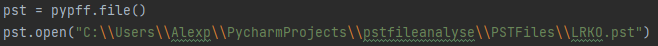
\includegraphics[width=0.75\textwidth]{images/File_open_libpff.PNG}
    \caption{Python Code - Öffnen der .pst-Datei mithilfe von libpff} 
    \label{fig:fileopen}
\end{figure}

\begin{figure}
    \centering
    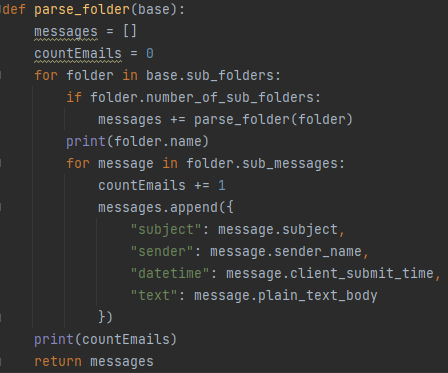
\includegraphics[width=0.75\textwidth]{images/Extraktion_aus_Pst_file.PNG}
    \caption{Python Code - Extraktion der Eigenschaften aus .pst-Datei} 
    \label{fig:extraction}
\end{figure}

\begin{figure}
    \centering
    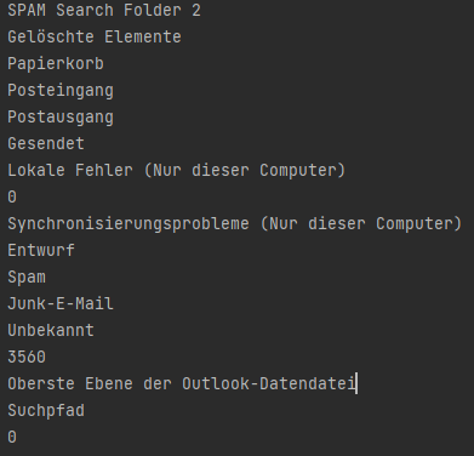
\includegraphics[width=0.50\textwidth]{images/PST_File_Aufbau_Python.png}
    \caption{Print Ausgabe - Aufbau der .pst-Datei} 
    \label{fig:pstfileaufbau}
\end{figure}

\begin{figure}
    \centering
    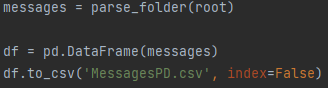
\includegraphics[width=0.75\textwidth]{images/Dataframe_messages.PNG}
    \caption{Python Code - Export in .CSV Datei} 
    \label{fig:dataframeparstetocsv}
\end{figure}

\begin{figure}
    \centering
    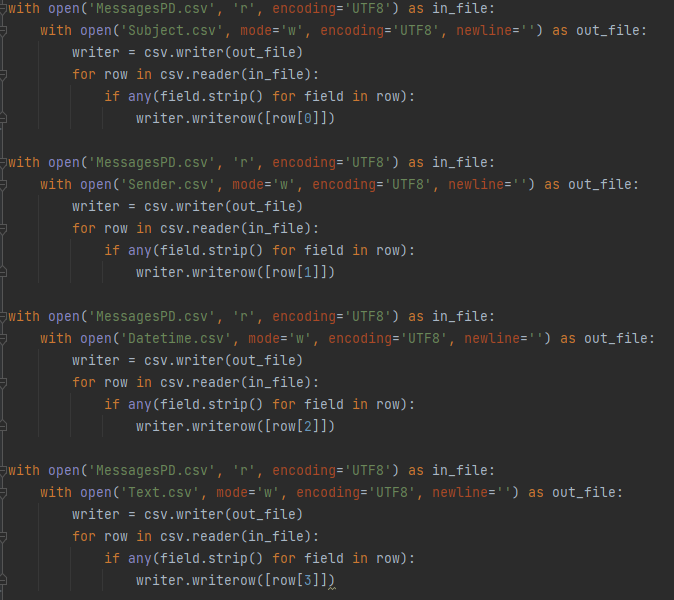
\includegraphics[width=0.75\textwidth]{images/Einzelne_Eigenschaften_in_CSV.PNG}
    \caption{Python Code - Extrahieren der einzelnen Eigenschaften in separate .csv-Dateien} 
    \label{fig:csvseparation}
\end{figure}
\label{Parsing der PST-Datei}

\subsection{Senderanalyse}
Eine Analyse der Sender wurde durchgeführt, um festzustellen, wie viele verschiedene Absender einer E-Mail an das analysierte Postfach gesendet haben und welche davon am häufigsten vorhanden waren. Bei dieser Analyse wurde die Eigenschaft \glqq{}sender\grqq{} der E-Mails betrachtet. Hierfür wurde eine Funktion \glqq{}get\_sender\_from\_csv\_file\grqq{} definiert. Diese Funktion durchläuft die .csv-Datei mit einer for-Schleife wobei geprüft wird, ob die Mail-Adresse der entsprechenden Zeile bereits in den Daten vorhanden war oder nicht und der Zähler dieser Zeile erhöht. Falls ein Eintrag noch nicht vorhanden war, wird ein neuer Eintrag in der Liste erstellt und weiter gesucht. Der restliche Code in diesem Skript dient dazu, eine .csv-Datei zu erstellen mit den Spalten \glqq{}Sender\grqq{} und \glqq{}Received Mails\grqq{} und die gezählten Emails in diese Datei einzutragen. Der Code für das Python-Skript ist in Abbildung \ref{fig:countemailssender} abgebildet. \newline
Der daraus entstandene Graph wurde auch hier wieder per Import der .csv-Datei in eine Excel Arbeitsmappe erstellt. Auf der Abbildung \ref{fig:receivedemails} wurden nur die Absender mit mehr als 30 Treffern abgebildet, um die Übersicht zu behalten. Erkennbar ist Facebook mit 752 Treffern und Lidl Insider mit 250 Treffern. Die Sender auf Platz 5 und 7 wurden aus Gründen des Datenschutzes entfernt. Als Dritter in der Liste war Web.de mit 192 Treffern sehr auffällig. Dies liegt daran, dass ein FreeMail Postfach verwendet wird und deshalb ständig \glqq{}Info-Mails\grqq{} vom Mail-Anbieter im Postfach auftauchen. Insgesamt waren in dem E-Mail Postfach 714 verschiedene Absender bei einer gesamten Anzahl von 4102 E-Mails vorhanden. Dabei ist mir aufgefallen, dass auch vermehrt gleiche Absender mit Variationen ihrer Senderinformationen vorhanden waren und somit nicht als gleicher Absender erkannt wurden. Erstaunlich ist, dass Lidl Insider mit 250 Treffern vorkommt, obwohl über das Postfach nur eine Bestellung bei Lidl getätigt wurde. Facebook tritt so oft auf, da der Nutzer des Postfachs seine E-Mail Benachrichtigungen aktiviert hat. Somit machte Facebook 18\% aus, Lidl Insider 6\% und Web.de immerhin noch ca. 4.5\%. \newline
Der zweite Graph (siehe Abbildung \ref{fig:receivedemailsmerged}) entstand aus einem Datensatz mit 6692 E-Mails. In dieser .pst-Datei waren insgesamt 148 verschiedene Absender von Mails vorhanden. Auch hier wurden die Absender mit mehr als 30 gesendeten E-Mails abgebildet. Sehr auffällig ist, dass es weniger Absender mit dieser Anzahl an gesendeten Mails gibt. Des Weiteren ist auffällig, dass die Absender weniger mit Spam zu tun haben, sondern vielmehr mit tatsächlich getätigten Transaktionen. Dies kommt daher, dass die zusammengesetzten .pst-Dateien aus E-Mail Konten stammen, die regelmäßig gepflegt werden und auch mit einem guten Spamfilter versehen sind. Ein Ausreißer mit 5653 gesendeten E-Mails wird hier nicht abgebildet, da er sonst die Grafik unnötig verzerren würde. Diese hohe Anzahl an Mails wurde von \glqq{}Twitch\grqq{} gesendet und es handelt sich dabei größtenteils um Benachrichtigungen des Dienstes, die man auch abschalten kann. Somit ist auch daran erkennbar, dass man ein Postfach gut sauber halten kann, wenn man die richtigen Mechanismen einführt bzw. unnötige Benachrichtigungen deaktiviert.



\begin{figure}
    \centering
    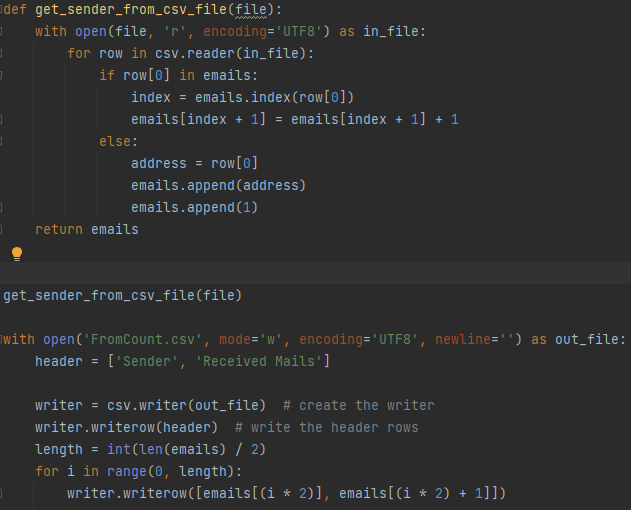
\includegraphics[width=0.75\textwidth]{images/Count_Received_Mails_Count_Sender.PNG}
    \caption{Python Code - Zählen der erhaltenen E-Mails und auflisten nach Absender} 
    \label{fig:countemailssender}
\end{figure}

\begin{figure}
    \centering
    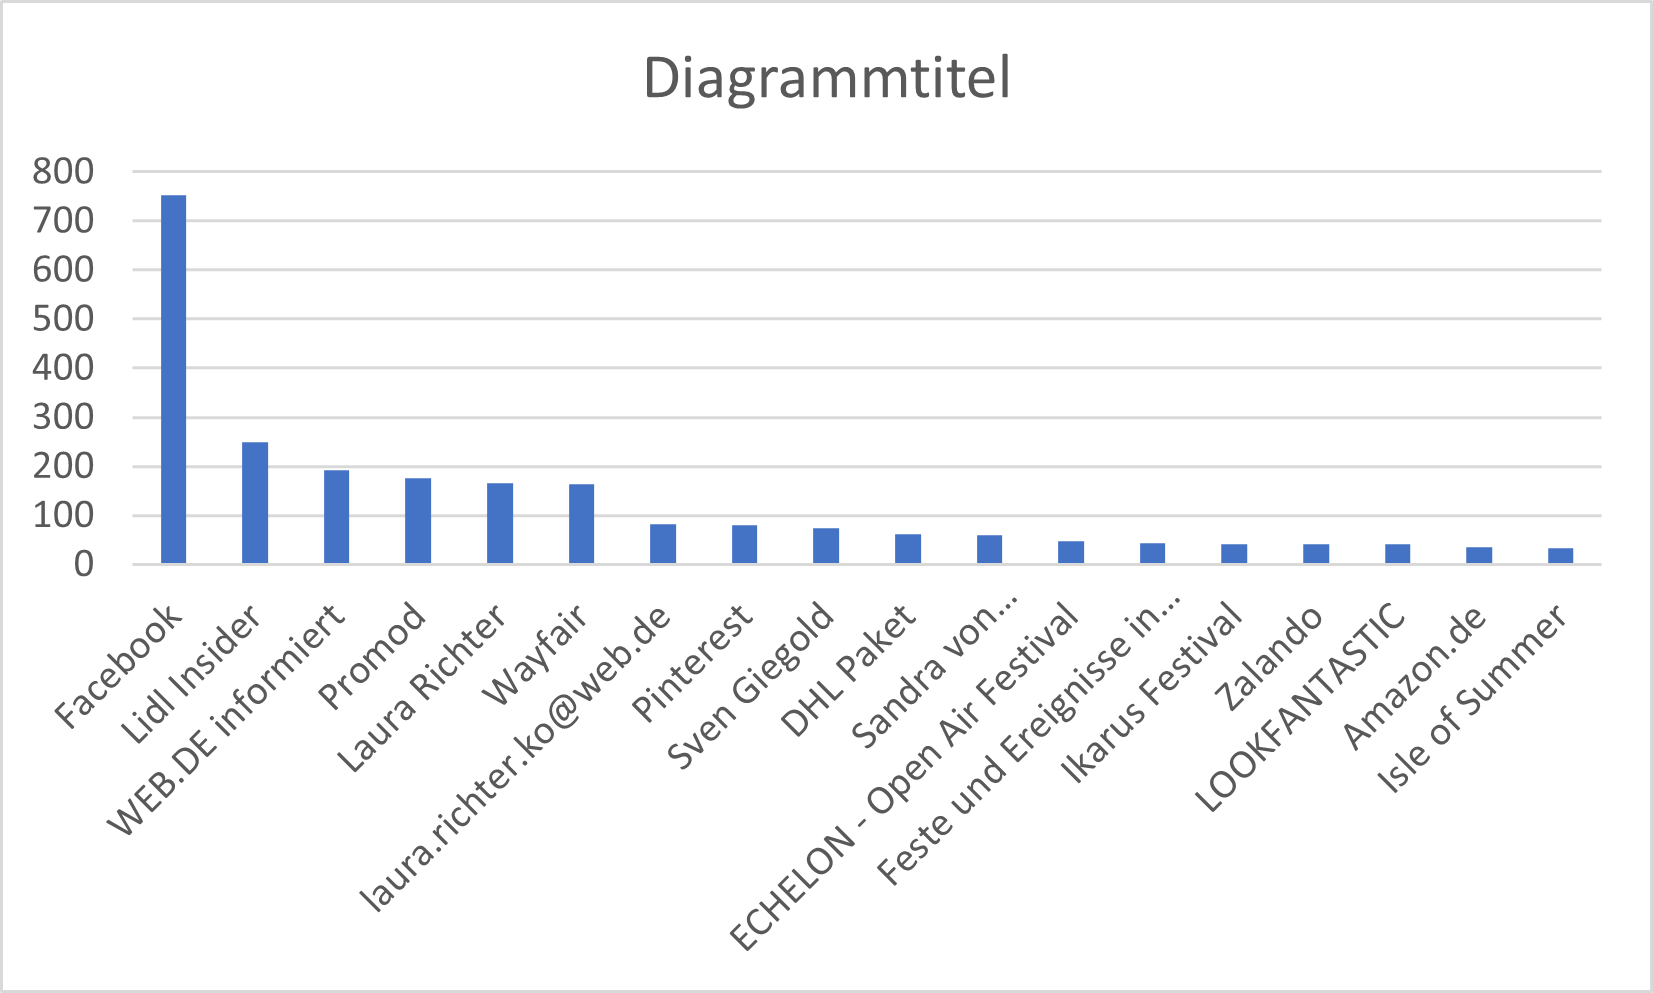
\includegraphics[width=0.75\textwidth]{images/Auswertung_Empfange_Emails.png}
    \caption{Absender mit mehr als 100 gesendeten Mails - Datensatz mit 4102 E-Mails} 
    \label{fig:receivedemails}
\end{figure}

\begin{figure}
    \centering
    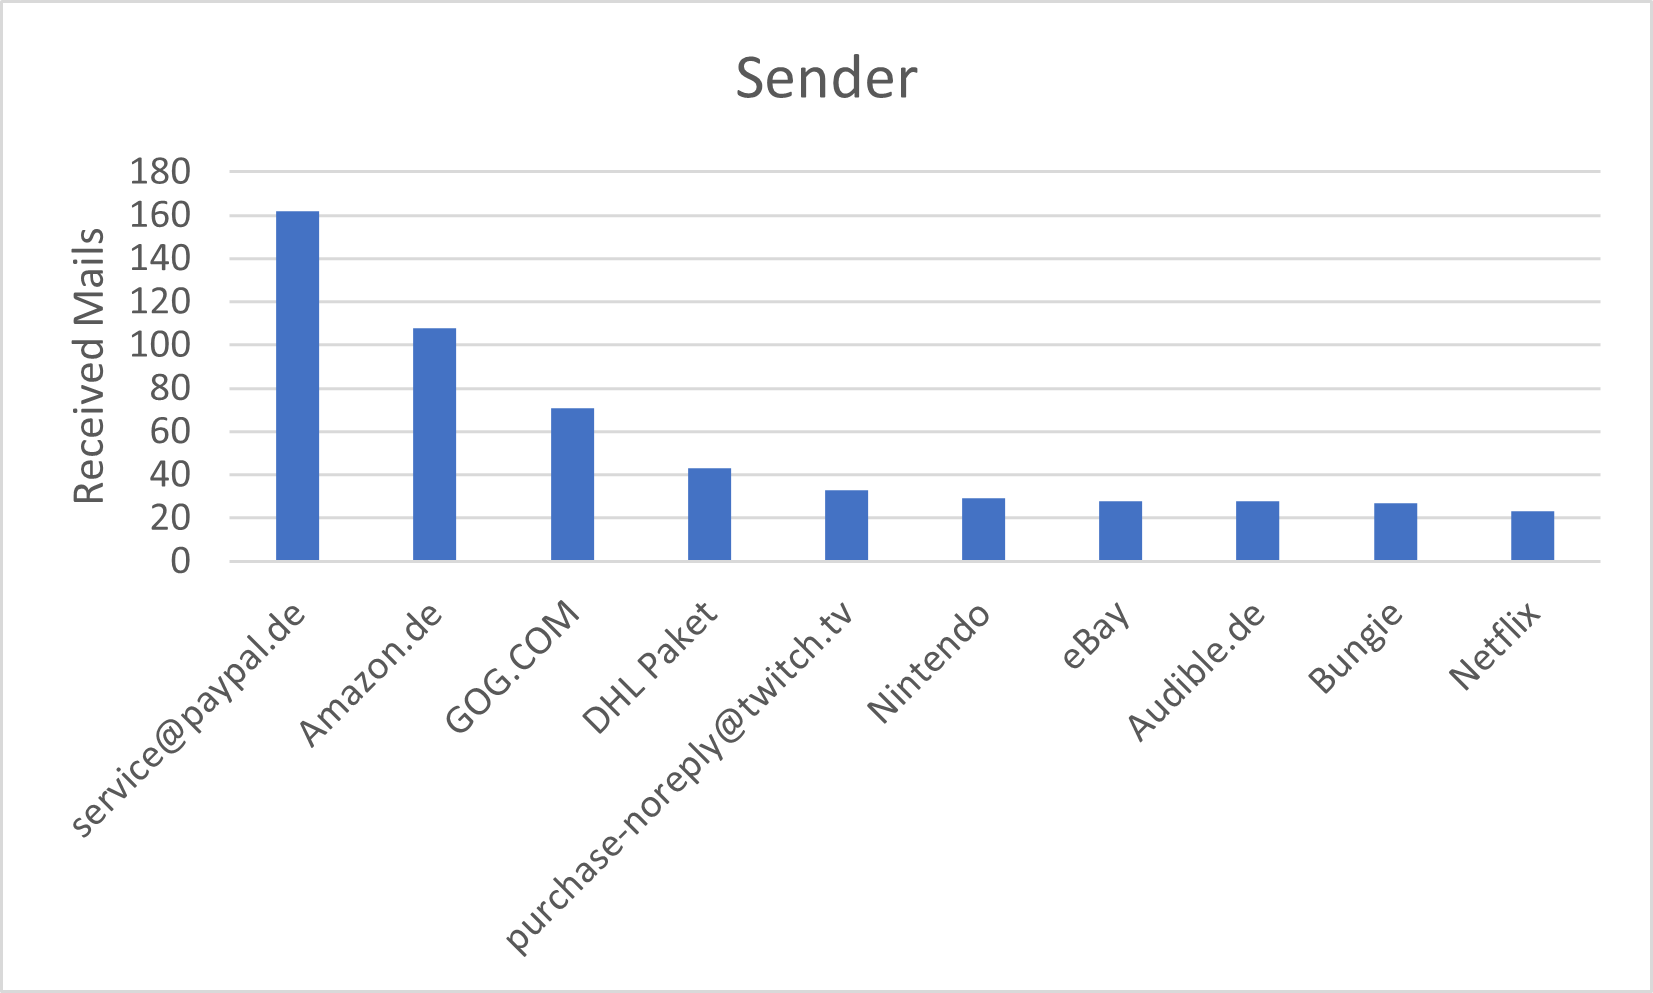
\includegraphics[width=0.75\textwidth]{images/Merged_Auswertung_Empfange_Emails.png}
    \caption{Absender mit mehr als 100 gesendeten Mails - Datensatz mit 6692 E-Mails} 
    \label{fig:receivedemailsmerged}
\end{figure}
\label{Senderanalyse}

\subsection{Zeitliche Analyse}
Die nächste Analyse bezieht sich auf das zeitliche Eintreffen von Emails. Durch das Parsen der .pst-Datei lag die Eigenschaft \glqq{}datetime\grqq, welche das Datum und die Zeit der empfangenen E-Mail darstellt in dem Format vor, dass in Abbildung \ref{fig:datetime} zu sehen ist. Mithilfe des Python Codes aus Abbildung \ref{fig:emailsdatetime} werden die Daten in die korrekte Zeitzone konvertiert, weil sie standardmäßig im UTC-Format gespeichert werden. Hierzu wird die Zeitzone erst als UTC deklariert und dann in die gewünschte Zeitzone umgewandelt. Im nachfolgenden Schritt werden die extrahierten Daten als Punktewolke, welche die Ankunftszeiten der E-Mails nach Datum darstellt, geplottet. Dazu werden zwei Spalten mit den Koordinaten der zu verfolgenden Punkte erstellt. Als letzter Schritt wird dann die Punktewolke erstellt. Dazu wurden die Python Bibliotheken \glqq{}matplotlib\grqq{} und \glqq{}seaborn\grqq{} verwendet. In dieser Seminararbeit wurde der vorhandene Datensatz vom Jahr 2020 bis Mitte 2022 analysiert. \newline
Daraus entstand der Graph, der in Abbildung \ref{fig:auswertungzeitlich} abgebildet wird. Klar erkennbar ist hier die Häufung von empfangenen E-Mails zwischen 16 und 18 Uhr. Ebenso ist ab dem Jahr 2022 eine Häufung der Nachrichten im Bereich um 14 bis 15 Uhr erkennbar. Auffällig ist, das zwischen 22 Uhr und 5 Uhr fast keine E-Mails eingetroffen sind. Daraus lässt sich ableiten, dass tatsächlich fast nur Mails gesendet zu Zeiten gesendet werden, bei denen der Nutzer auch selbst aktiv ist. \newline
Die Punktewolke, die sich aus dem zweiten Datensatz ableiten lässt, ist in Abbildung \ref{fig:auswertungzeitlichmerged} zu sehen. Hier ist anzumerken, dass die zeitliche Verteilung leider wenig Aussagekräftig ist, da unter Berücksichtigung aller empfangener E-Mails die hohe Anzahl an Benachrichtigungen von \glqq{}Twitch\grqq{} enthalten ist und diese zu jeder Tages- und Nachtzeit auftreten. Beim herausfiltern all dieser E-Mails waren keine besonderen zeitlichen Auffälligkeiten der anderen Mails erkennbar, da es dafür wiederum zu wenige über den betrachteten Zeitraum waren, wobei dieser sogar schon auf die erste Hälfte des Jahres 2022 eingeschränkt wurde. 

\begin{figure}
    \centering
    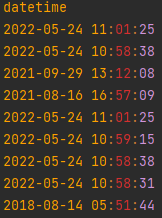
\includegraphics[width=0.50\textwidth]{images/datetime.PNG}
    \caption{E-Mail Eigenschaft datetime} 
    \label{fig:datetime}
\end{figure}

\begin{figure}
    \centering
    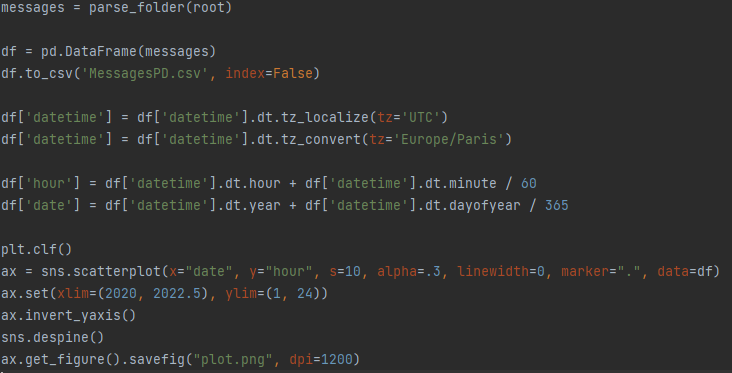
\includegraphics[width=0.75\textwidth]{images/Auswertung_Zeiten.PNG}
    \caption{Python Code - Auswertung hinsichtlich der Empfangszeiten} 
    \label{fig:emailsdatetime}
\end{figure}

\begin{figure}
    \centering
    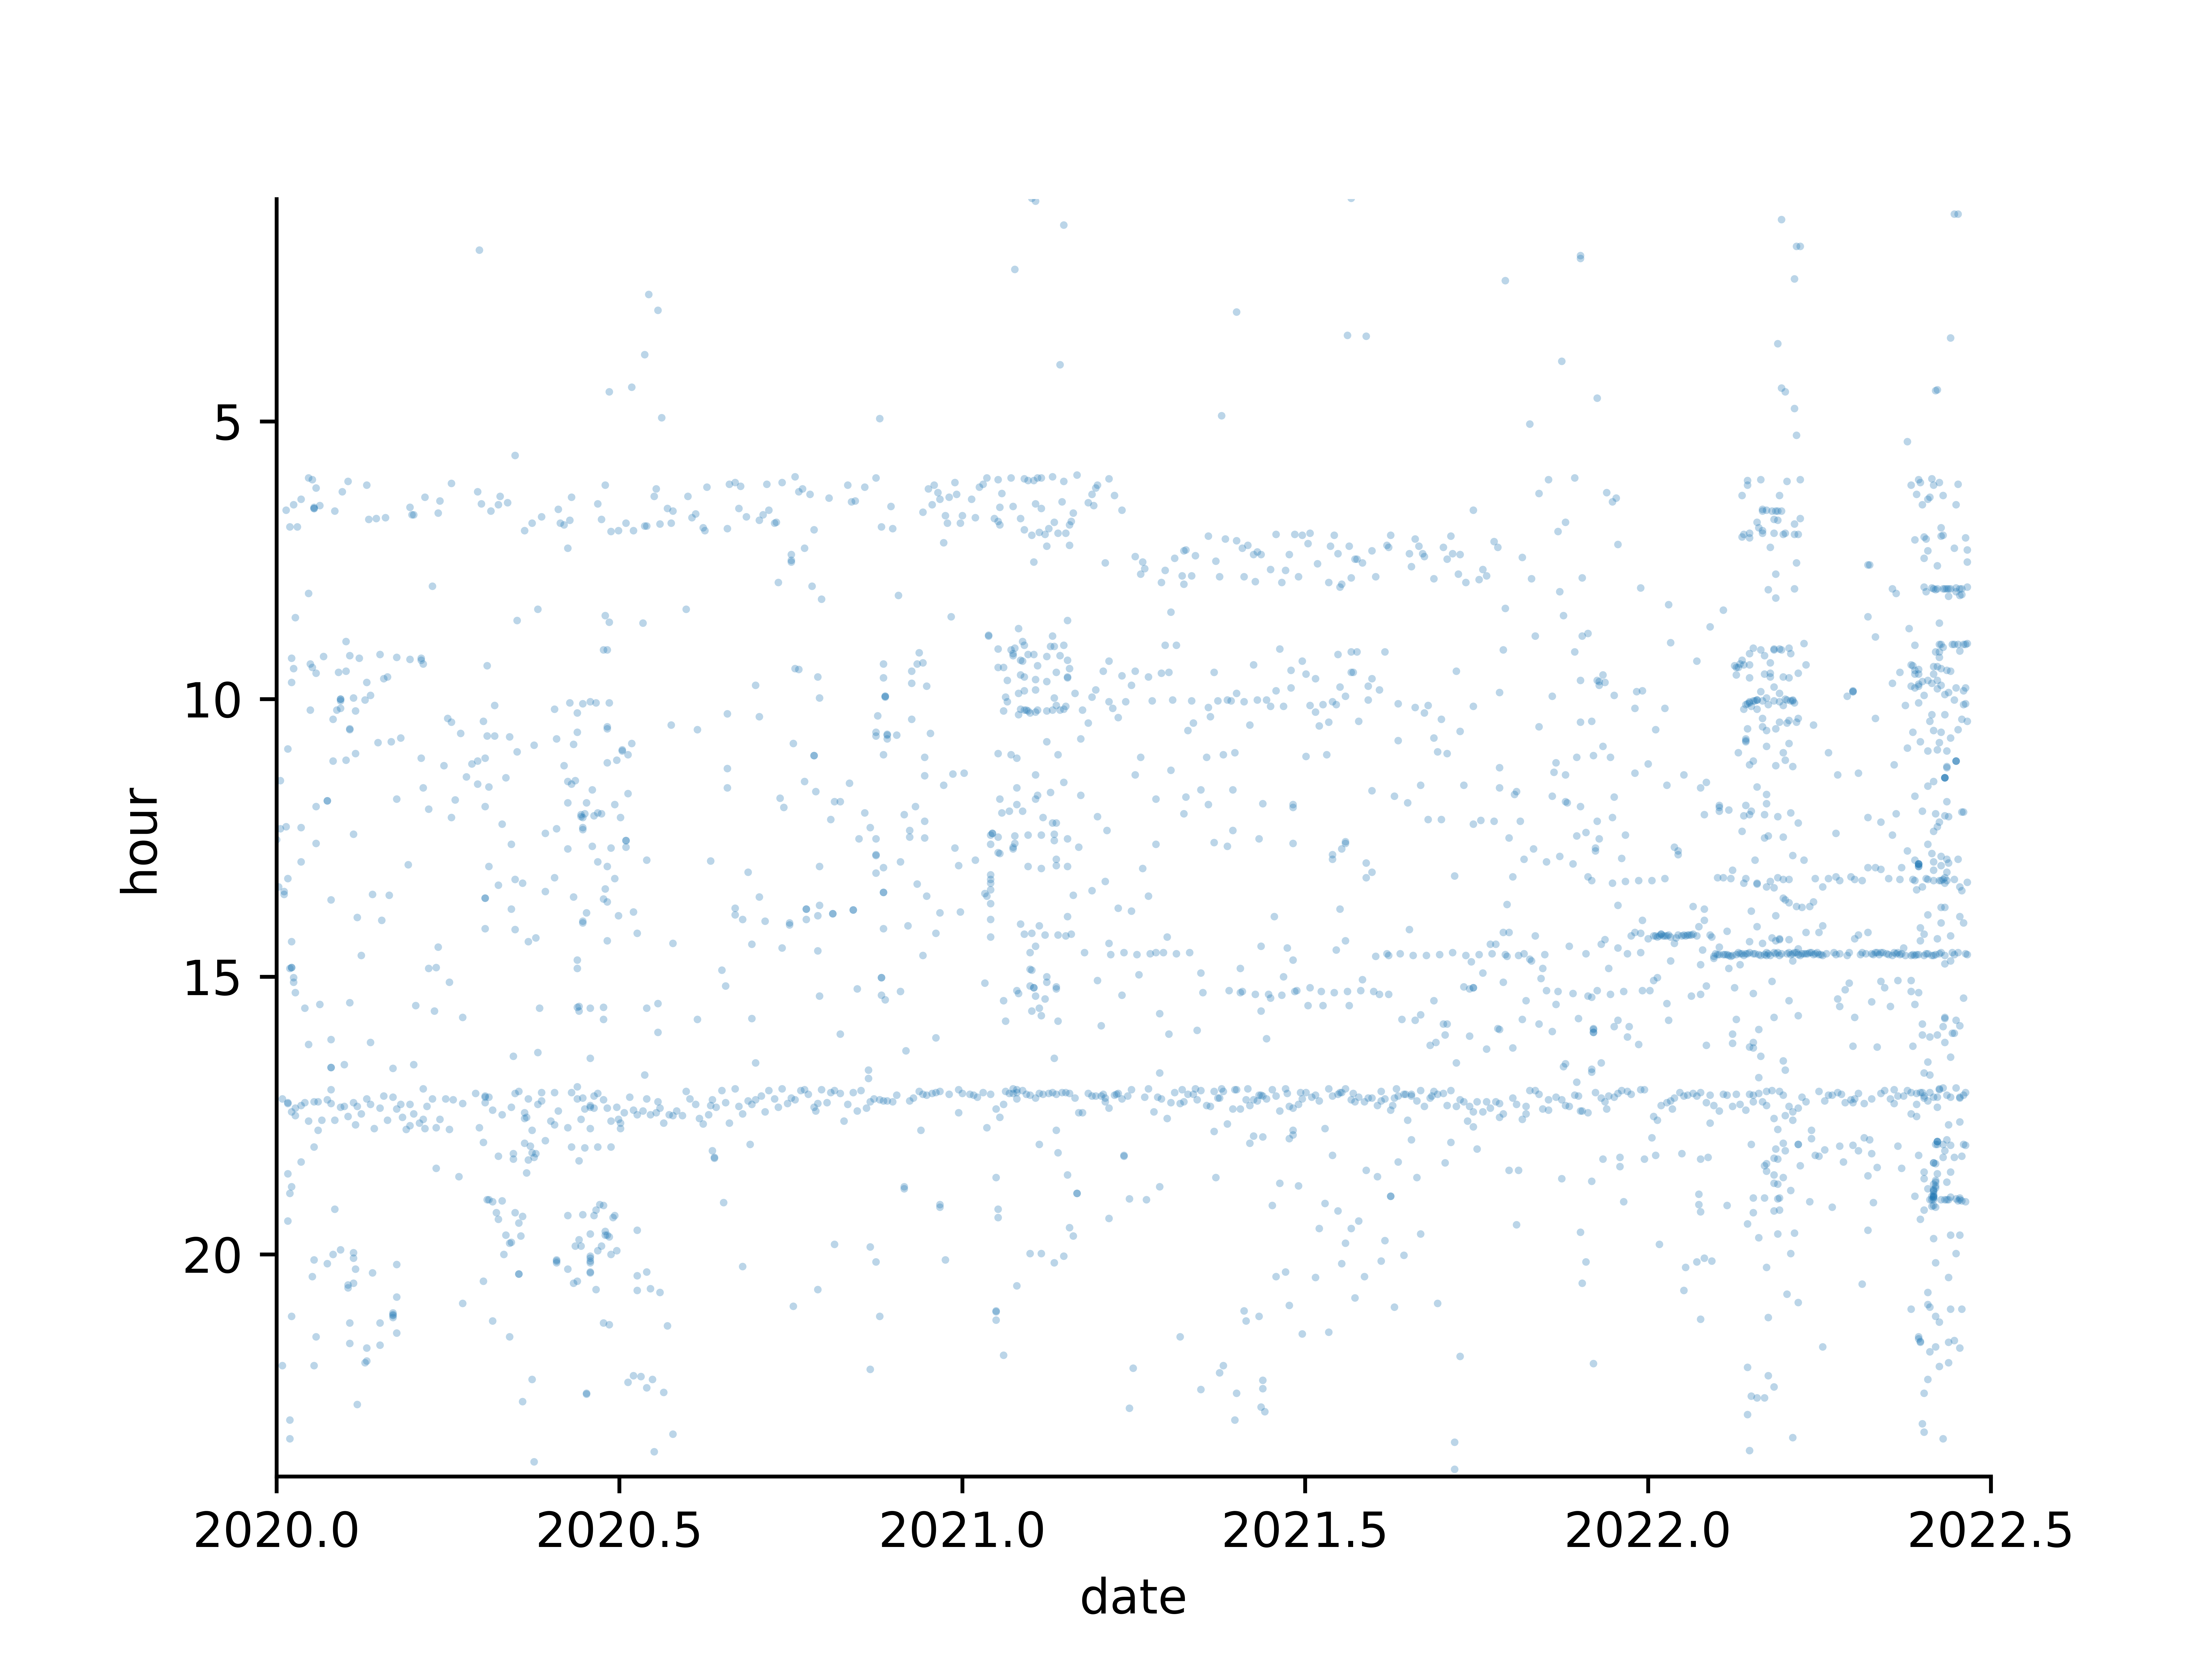
\includegraphics[width=0.75\textwidth]{images/plot.PNG}
    \caption{Zeitliche Verteilung der E-Mails} 
    \label{fig:auswertungzeitlich}
\end{figure}


\begin{figure}
    \centering
    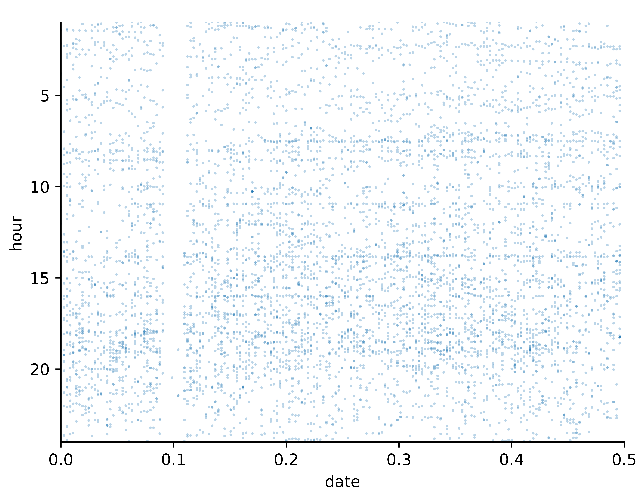
\includegraphics[width=0.75\textwidth]{images/merged_plot.PNG}
    \caption{Zeitliche Verteilung der E-Mails bei zusammengesetztem Postfach} 
    \label{fig:auswertungzeitlichmerged}
\end{figure}
\label{Zeitliche Analyse}

\subsection{Analyse von Spam-Wörtern}
In diesem Kapitel wird auf die Analyse bestimmter Schlagwörter in den E-Mails eingegangen. Um diese Analyse durchzuführen habe ich im Internet nach gängigen Wörtern gesucht, die auf eine Spam-Mail hinweisen \cite{Heise.07.06.2021}. Anhand der gefundenen Wörter habe ich passende ausgesucht und als Liste in einem Python Skript hinterlegt. Diese Liste ist in Abbildung \ref{fig:spamwortliste} zu sehen und enthält 176 Schlagwörter. Dabei wurden Kategorien wie Finanzen, Glücksspiel, Gesundheit, Shopping, Dating und Sonstige betrachtet. Für die Analyse der Wörter wurde die .csv-Datei verwendet, welche beim Parsen der .pst-Datei entstanden ist. Diese wurde dann mit je einem Wort aus der Spamwort-Liste durchlaufen und ein Counter erhöht, sobald ein Treffer erzielt wurde. Anschließend wurde die Liste \glqq{}word\_list\grqq{} mit den Headern \glqq{}SpamWords\grqq{} und \glqq{}Hits\grqq{} in eine .csv-Datei exportiert um eine grafische Auswertung dieser Daten vorzunehmen. Der hierfür verwendete Python Code ist in Abbildung \ref{fig:spamwordsearch} zu sehen. Die hierdurch erstellte .csv-Datei habe ich im Anschluss in Microsoft Excel importiert und dort eine Graphische Auswertung durchgeführt. Excel habe ich gewählt, da ich anders als bei der Auswertung der zeitlichen Eigenschaften der E-Mails eine andere Art der grafischen Auswertung abseits von Python ausprobieren wollte. \newline
Das Ergebnis der Auswertung ist in Abbildung \ref{fig:spamwortlistegreater100} zu sehen. Am häufigsten kamen davon das Wort \glqq{}Angebot\grqq{} mit 5092 Treffern, danach \glqq{}Date\grqq{} mit 2991 Treffern gefolgt von \glqq{}klicken\grqq{} mit 1319 Treffern vor. Diese Wörter sind in die Kategorien Shopping und Dating sowie Sonstige einzuordnen. In der Abbildung \ref{fig:spamwortlistegreater100} sind alle Wörter mit einer Trefferanzahl von mehr als 100 abgebildet. \newline 
Im zweiten Datensatz wurden ebenfalls alle Wörter mit mehr als 100 Treffern abgebildet (\ref{fig:spamwortlistegreater100merged}). Dabei war das Wort \glqq{}Date\grqq{} auch hier sehr oft vertreten und zwar mit 1027 Treffern. Danach folgt das Wort \glqq{}Angebot\grqq{} mit 716 Treffern. Die zwei Wörter mit den höchsten Treffern sind also identisch zum anderen Datensatz. Auf beiden Grafiken zur Auswertung der Spamwortsuche ist auch erkennbar, dass sich die Wörter mit über 100 Treffern überschneiden. Somit lässt sich zumindest anhand dieser beider .pst-Dateien ein Muster an häufig auftretenden Schlagworten erkennen. 

\begin{figure}
    \centering
    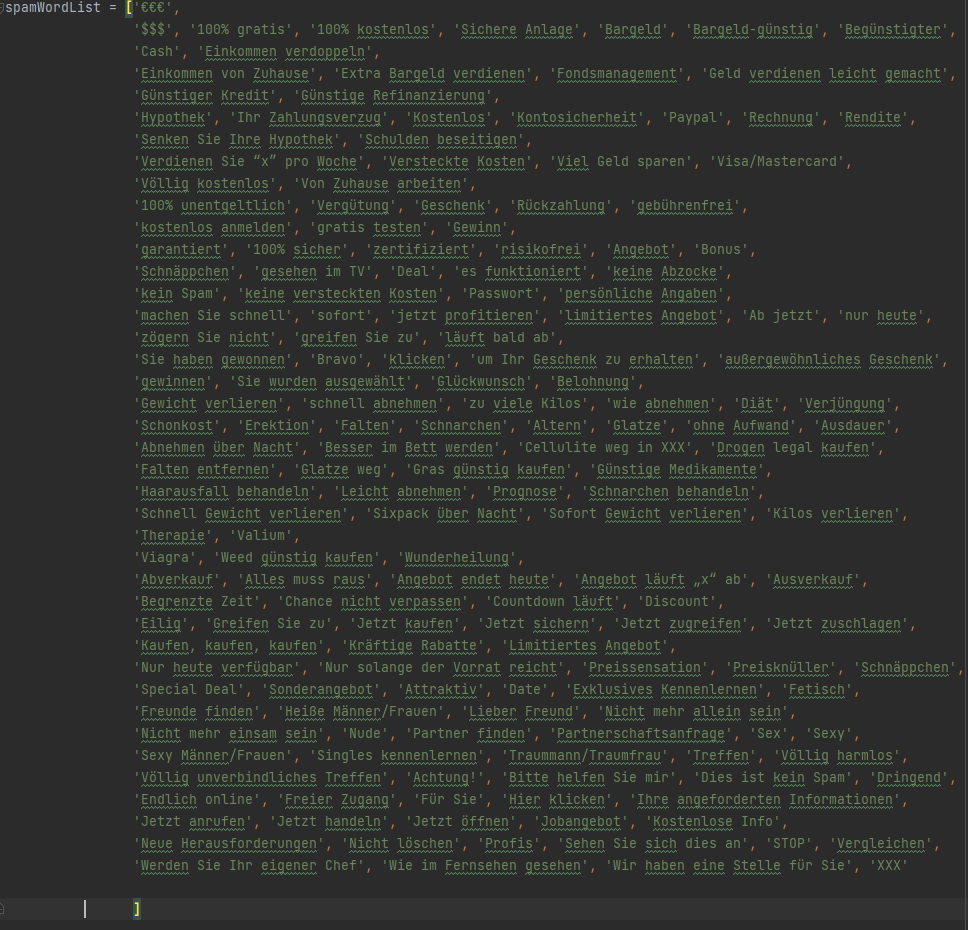
\includegraphics[width=0.75\textwidth]{images/Spamwortliste.PNG}
    \caption{Spamwortliste} 
    \label{fig:spamwortliste}
\end{figure}

\begin{figure}
    \centering
    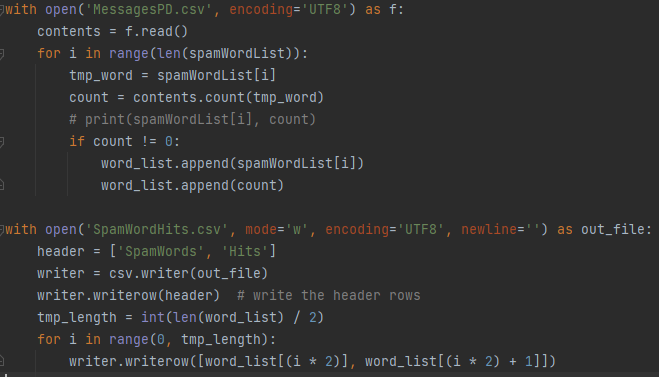
\includegraphics[width=0.75\textwidth]{images/python_Spamwordsearch.PNG}
    \caption{Python Code - Durchsuchen der E-Mails nach Schlagworten} 
    \label{fig:spamwordsearch}
\end{figure}

\begin{figure}
    \centering
    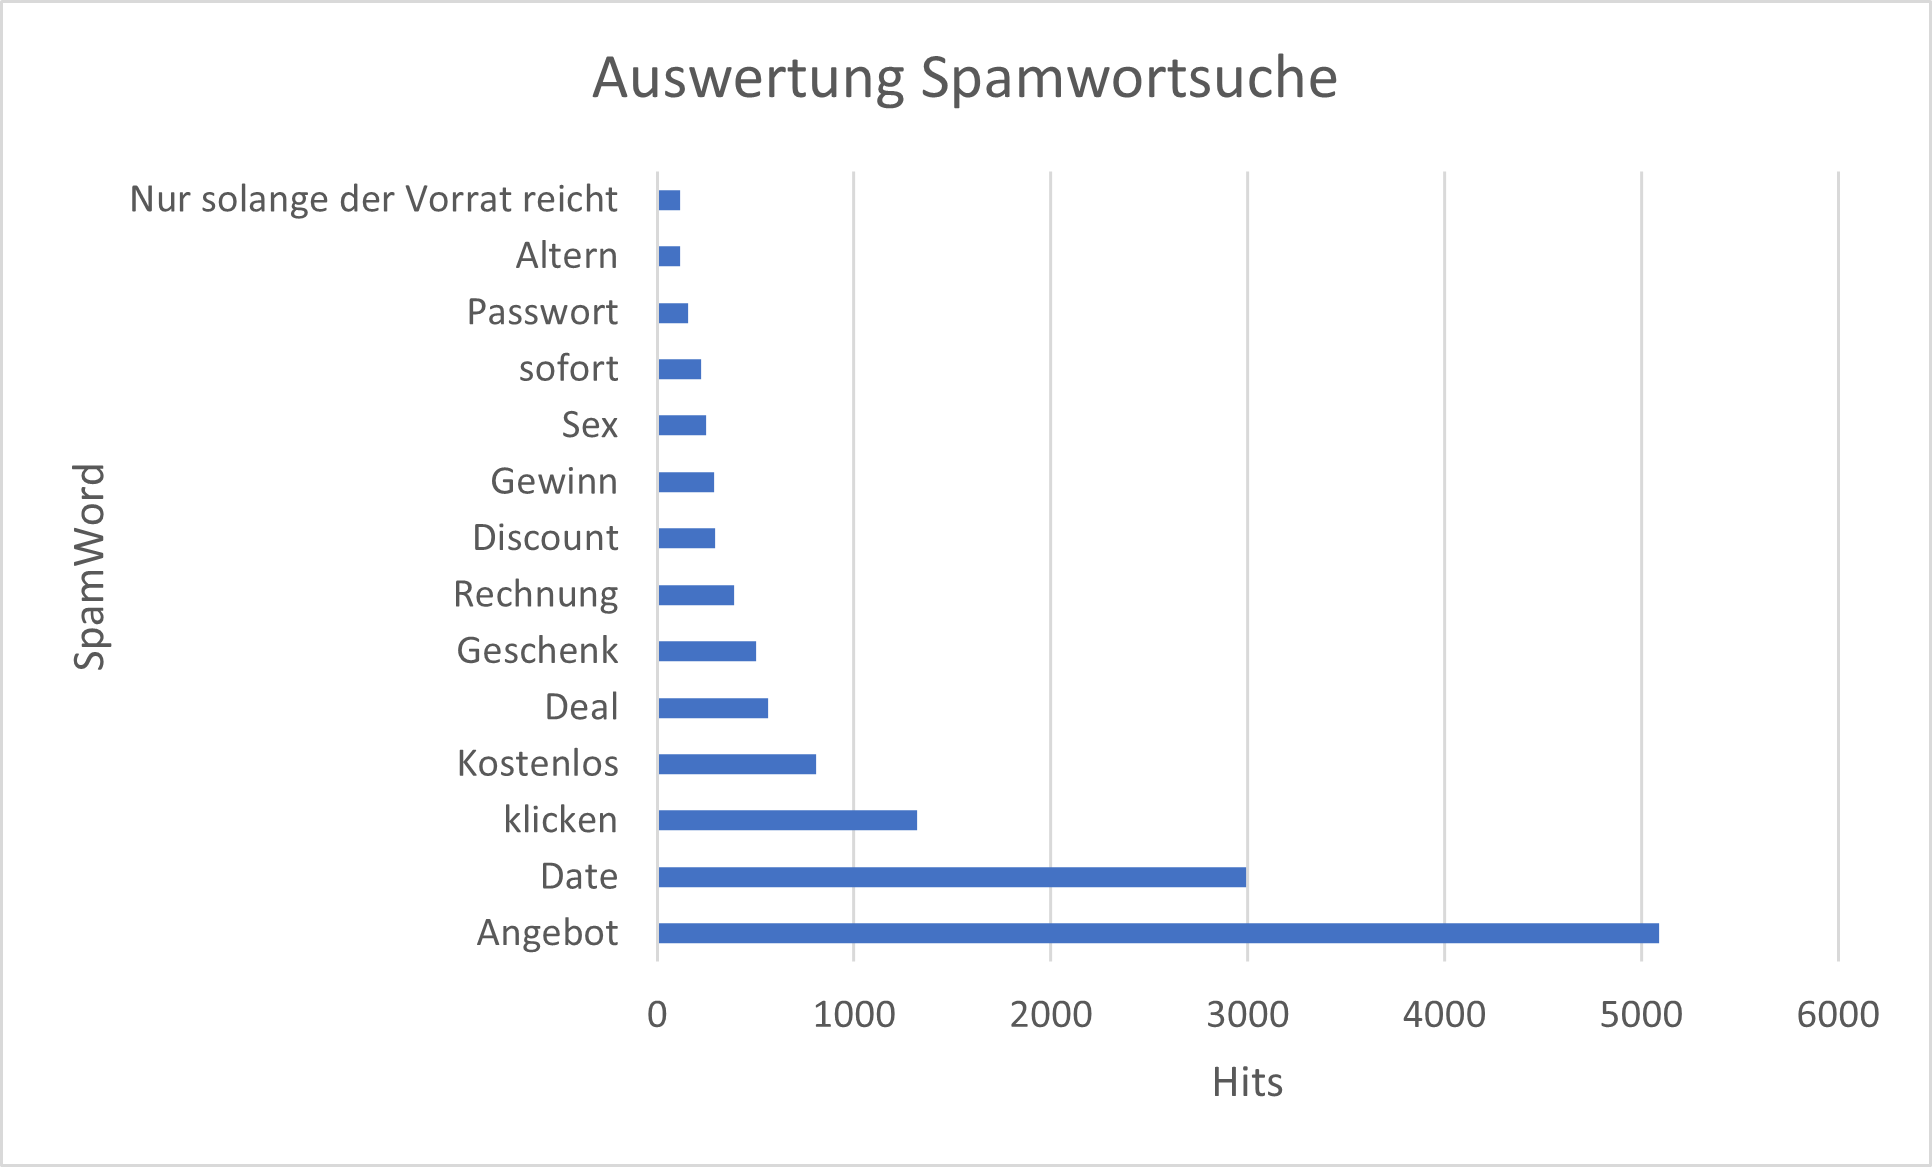
\includegraphics[width=0.75\textwidth]{images/Auswertung_Spamwortsuche.png}
    \caption{Wörter mit mehr als 100 Treffern - Datensatz mit 4102 E-Mails} 
    \label{fig:spamwortlistegreater100}
\end{figure}


\begin{figure}
    \centering
    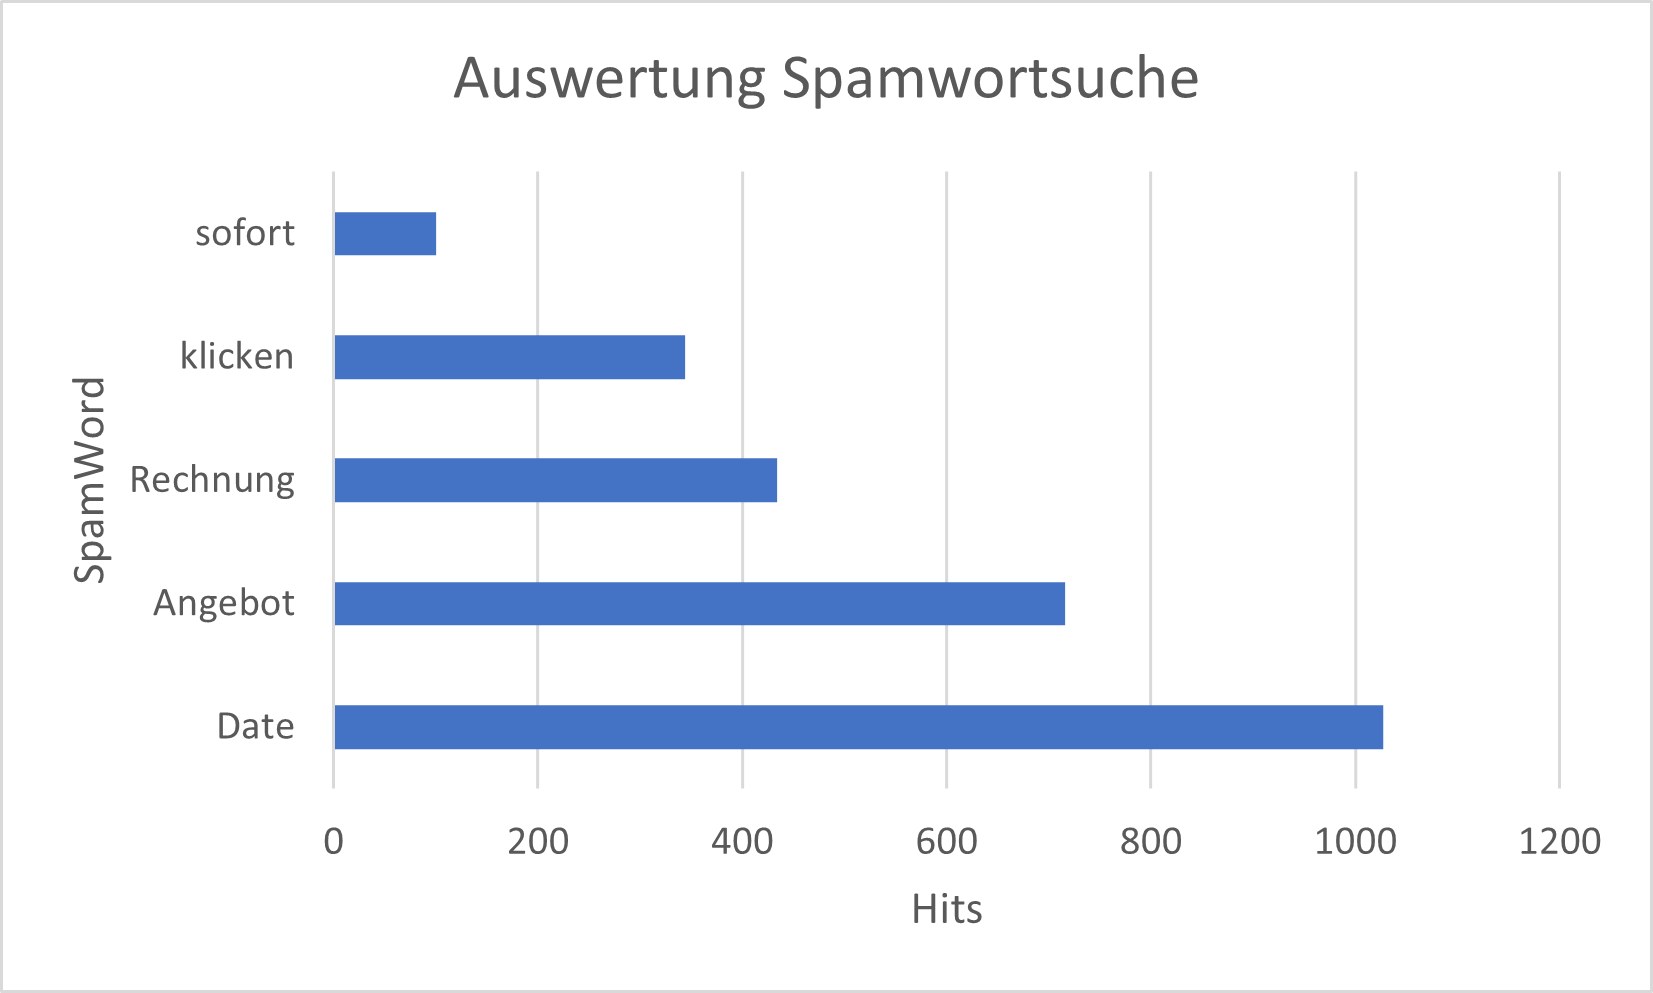
\includegraphics[width=0.75\textwidth]{images/Merged_Auswertung_Spamwortsuche.png}
    \caption{Wörter mit mehr als 100 Treffern - Datensatz mit 6692 E-Mails} 
    \label{fig:spamwortlistegreater100merged}
\end{figure}
\label{Analyse von Spam-Wörtern}

\section{Ergebnisse}
In diesem Kapitel werden die Ergebnisse der Analyse näher erläutert.
\label{Ergebnisse}

\section{Fazit}
In dieser Seminararbeit wurde eine forensische Analyse einer .pst-Datei durchgeführt. Hierfür wurden verschiedene Analysen durchgeführt. Die Analysen wurde mithilfe von eigens geschriebenen Python-Skripten durchgeführt, da Tools für die Analyse von .pst-Dateien nur kostenpflichtig zur Verfügung standen bzw. die kostenfreien Versionen nur sehr eingeschränkte Funktionalitäten besessen haben. Durch die Verwendung professioneller Tools wären mit großer Wahrscheinlichkeit noch viel detailliertere Ergebnisse zustande gekommen. Zum Parsing der .pst-Datei wurde die Python Bibliothek "libpff" verwendet, die sich speziell für den Zugriff auf Dateiformate von Microsoft Outlook eignet. Mithilfe dieser Bibliothek wurden dann die wichtigsten Eigenschaften der E-Mails extrahiert, um sie für die weitere Analyse aufzubereiten. \newline
Im Anschluss daran wurden dann eine Senderanalyse, eine zeitliche Analyse und eine Spamwortanalyse durchgeführt. Die Senderanalyse hat gezeigt, dass Facebook mit 752 E-Mails auf Platz 1 der meisten gesendeten E-Mails liegt. Dies liegt höchstwahrscheinlich daran, dass der Besitzer des Postfaches seine Facebook Benachrichtigungen aktiviert hat. Auf dem zweiten Platz liegt jedoch "Lidl Insider" mit 250 E-Mails. Dieses Ergebnis ist erschreckend, da ich nach einer Rücksprache mit dem Besitzer des E-Mail Kontos erfahren habe, dass genau eine Bestellung vor einigen Jahren durchgeführt wurde und seitdem zahlreiche E-Mails mit Werbung empfangen werden. Die Analyse der Empfangszeiten der E-Mails hat gezeigt, dass deutliche Muster von Häufungen der empfangenen E-Mails zu bestimmten Zeiträumen erkennbar sind. In dem verwendeten Datensatz war klar erkennbar, dass sich eine Häufung zwischen 16 und 18 Uhr abzeichnet. Dies ist für viele Personen die Zeit um Feierabend zu machen. Das ist insofern eine gute Zeit, da viele Leute dann erschöpft und somit unvorsichtiger sind und leichter auf eine Spam-Mail hereinfallen. Bei der Analyse der auftretenden Spam-Wörter in den E-Mails wurde eine mithilfe häufig verwendeter Wörter eine \glqq{}Spam-Wort-Liste\grqq{} erstellt. Die Inhalte der E-Mails wurden dann mit der Liste überprüft, um zu sehen wie häufig bestimmte Wörter auftreten. Dabei war \glqq{}Angebot\grqq{} mit 5092 Treffern klar auf Platz 1 und \glqq{}Date\grqq{} mit 2991 Treffern auf Platz 2. Somit kam das Wort Angebot im Schnitt in 1,2 E-Mails vor. \newline
Zu erwähnen ist jedoch, dass diese Ergebnisse nicht repräsentativ sind. Um bessere Ergebnisse zu erzielen bräuchte man zum Einen mehr E-Mails und zum Anderen mehrere E-Mail Konten verschiedener Benutzer, um andere Verhaltensmuster im zu analysierenden Datensatz vorzufinden.\newpage
\label{Fazit}

\bibliographystyle{plain}
\bibliography{literaturverzeichnis/literaturverzeichnis}

\end{document}
